% SVN info for this file
% SVN info for this file
\svnidlong
{$HeadURL$}
{$LastChangedDate$}
{$LastChangedRevision$}
{$LastChangedBy$}

\chapter{Il potenziale elettrico e le leggi di Maxwell per l'elettrostatica} %TODO: Il lavoro elettrico?
%TODO: tcbox
\labelChapter{PotenzialeElettrico}
\begin{introduction}
	``Una volta che ti pompano 200 volt nel corpo, hai la tendenza a passare il resto della vita in un posacenere.''
	\begin{flushright}
		\textscsl{Woody Allen}, elettricista con la carriera andata in fumo.
	\end{flushright}
\end{introduction}
\lettrine[findent=1pt, nindent=0pt]{C}{ome} abbiamo visto negli esempi del \autoref{chap:FlussoCampoElettrico}, il campo elettrostatico $\vba{E}$ non è una funzione vettoriale come tutte le altre, ma è un campo \textit{conservativo} - non nel senso politico del termine, dato che i campi vettoriali non hanno diritto di voto. Ciò che intendiamo con ciò è che esso ammette una funzione scalare $V$ per cui $\vba{E}$ è il gradiente di $V$. Oltre ad avere importanti conseguenze fisiche, il potenziale ci permette una \textit{terza via} per calcolare i campi elettrostatici, dopo quella diretta con gli integrali e quella tramite la legge di Gauss: determinare il campo scalare potenziale e, prendendo il suo gradiente, ricavare quello elettrostatico.

In questo capitolo mostreremo cosa cambia nel passaggio dalle forze conservative ai \textbf{campi conservativi} (spoiler: ben poco, tutto sommato), introducendo il concetto di \textbf{circuitazione di un campo vettoriale}. Fatto ciò passeremo a parlare del \textbf{potenziale elettrico} e mostreremo attraverso alcuni esempi come si comporta in presenza di \textbf{discontinuità di campo elettrostatico}.\\
Concludiamo questa sezione reinterpretando i risultati di questi primi tre capitoli sotto forma delle \textbf{equazioni di Maxwell per l'elettrostatica}; inoltre, ci soffermeremo su particolari equazioni differenziali, dette \textbf{di Poisson} e \textbf{di Laplace}, con la quale possiamo semplificare ulteriormente lo studio del potenziale - e di conseguenza del campo elettrostatico.
\vfill
\pagebreak
\section{La circuitazione di un campo vettoriale}
\begin{define}[Circuitazione di un campo vettoriale]
La \textbf{circuitazione di un campo vettoriale lungo una curva chiusa}\index{circuitazione di un campo vettoriale} $\gamma$, parametrizzata da una funzione $\ \funz[\vba{r}]{\left[a,b\right]}{\realset^3}$, è\\
	\begin{minipage}{0.65\textwidth}
		\begin{equation}
			\tcboxmath[colback=yellowpastellow!30!white,colframe=ceruleancrayola!85!black,drop fuzzy shadow, nobeforeafter, math upper, tcbox raise base, enhanced]{\Gamma_{\gamma}(\vba{E})=\oint_{\gamma}\vba{E}\vdot d\vba{s}=\int_{a}^b\vba{E}\vdot\frac{d\vba{r}}{dt}dt}
		\end{equation}
	\end{minipage}\hspace{5pt}
	\begin{minipage}{0.34\textwidth}
		\begin{center}
			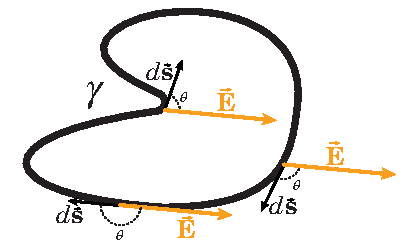
\includegraphics[width=1\textwidth]{images/chp3/chp3circuitazione.pdf}
		\end{center}
	\end{minipage}
\end{define}
\paragraph{Dalle forze conservative...}
La circuitazione ha particolare rilevanza in ambito fisico: la sua prima applicazione che vedremo è in una caratterizzazione dei\textit{campi vettoriali conservativi}. Prima però, riguardiamo rapidamente il concetto di lavoro e del suo ruolo per quelle forze dette \textit{forze conservatrici}, trattate nel corso di \textsc{Fisica I}.
\begin{define}[Lavoro]
	Dati due punti $\vba{r}_A$ e $\vba{r}_B$, il \textbf{lavoro}\index{lavoro} di una forza $\vba{F}$ lungo una curva $\gamma$ tra i due punti è definito come
	\begin{equation}
		\tcboxmath[colback=yellowpastellow!30!white,colframe=ceruleancrayola!85!black,drop fuzzy shadow, nobeforeafter, math upper, tcbox raise base, enhanced]{W_{\gamma_1}=\int_{\gamma_1}\vba{F}\vdot d\vba{s}}
	\end{equation}
\end{define}
In generale, il lavoro dipende dal \textit{percorso effettuato}: il lavoro compiuto da una stessa forza lungo due curve $\gamma_1$ e $\gamma_2$  è differente. Per un caso particolare di forze, tuttavia, il lavoro dipende esclusivamente dagli estremi e non dal percorso effettuato.
\begin{define}[Forza conservativa]
	Una forza $\vba{F}$ è detta \textbf{conservativa}\index{forza!conservativa} se per qualunque curva $\gamma_1,\ \gamma_2$ tra due punti $\vba{r}_A$ e $\vba{r}_B$ il lavoro è
	\begin{equation}
		\tcboxmath[colback=yellowpastellow!30!white,colframe=ceruleancrayola!85!black,drop fuzzy shadow, nobeforeafter, math upper, tcbox raise base, enhanced]{W_{\gamma_1}=W_{\gamma_2}}
	\end{equation}
	In altre parole, $\vba{F}$ è conservativa se il lavoro dipende \textit{solo} dai punti iniziali e finali e non quale sia la curva lungo la quale si calcola.
\end{define}
\begin{proposition}[Caratterizzazione delle forze conservative]\label{forzaconservativaproposizione}
	Se una forza $\vba{F}$ è conservativa, allora esiste una funzione scalare $\ \funz[U]{\realset^3}{\realset}$ detta \textbf{energia potenziale}\index{energia!potenziale} tale per cui\footnote{Il meno è presente per motivi storici.}
	\begin{equation}
		\vba{F}=-\grad{U}
	\end{equation}
	e tale per cui
	\begin{equation}
		W=U(\vba{r}_A)-U(\vba{r}_B)=-\Delta U
	\end{equation}
	In altri termini:
	\begin{gather}
		\vba{F}=-\grad{U}\\
		W=\int_A^{B}\vba{F}\vdot d\vba{s}=-\int_A^B\grad{U}\vdot d\vba{s}
	\end{gather}
\end{proposition}
\begin{observe}
	Questo non è altro che la ``versione fisica''  del \textbf{teorema del gradiente}. Nella ``Raccolta Differenziata'', a pag. \pageref{thmgradiente} è possibile trovare l'enunciato \textit{matematico} del teorema, dato che la dimostrazione è \textit{mutatis mutandis} quella che segue.
\end{observe}
\begin{demonstration}
	Consideriamo una curva $\gamma$ parametrizzata da
	\begin{equation*}
		\vba{r}(t)=\left(x(t),y(t),z(t)\right),\ \quad t\in\left[t_1,t_2\right]
	\end{equation*}
	Posto
	\begin{equation*}
		\begin{cases}
			\vba{r}(t_A)=\vba{r}_A\\
			\vba{r}(t_B)=\vba{r}_B
		\end{cases}
	\end{equation*}
si ha
\begin{align*}
	W&=\int_{t_A}^{t_B}\vba{F}\vdot\dv{\vba{r}}{t}dt=-\int_{t_A}^{t_B}\grad{U}\vdot\dv{\vba{r}}{t}dt=-\int_{t_A}^{t_B}\dv{t}U\left(\vba{r}(t)\right)dt=\\
	&=-\left(U(\vba{r}(t_B))-U(\vba{r}(t_A))\right)=U(\vba{r}_A)-U(\vba{r}_B)
\end{align*}
Infatti,
\begin{equation*}
	\dv{t}U(\vba{r}(t))=\pdv{U}{x^i}\pdv{x^i}{t}=\grad{U}\vdot\pdv{r}{t}.\qedhere
\end{equation*}
\end{demonstration}
\begin{observe}
	Il potenziale è sempre definito a meno di costante additiva. Infatti, se considero due potenziali $U$ e $U'=U+U_0$ dove $U_0$ è una costante reale, si ha che
	\begin{equation*}
		\vba{F}=-\grad{U'}=-\grad{(U+U_0)}=-\grad{U}-\underbrace{\grad{U_0}}_{=0}=-\grad{U}
	\end{equation*}
\end{observe}
\paragraph{...ai campi vettoriali conservativi}
In modo analogo a come abbiamo fatto per le forze conservative, possiamo facilmente definire un \textit{campo vettoriale conservativo}.
\begin{define}[Campo vettoriale conservativo]
	Una campo vettoriale $\vba{G}$ è detto \textbf{conservativo}\index{campo!conservativo} se per qualunque curva $\gamma_1,\ \gamma_2$ tra due punti $\vba{r}_A$ e $\vba{r}_B$ si ha
	\begin{equation}
		\tcboxmath[colback=yellowpastellow!30!white,colframe=ceruleancrayola!85!black,drop fuzzy shadow, nobeforeafter, math upper, tcbox raise base, enhanced]{\int_{\gamma_1}\vba{G}\vdot d\vba{s}=\int_{\gamma_1}\vba{G}\vdot d\vba{s}}
	\end{equation}
\end{define}
\begin{proposition}[Caratterizzazione dei campi vettoriali conservativi]\label{campivettorialiconservativiproposizione}
	Se un campo vettoriale$\vba{G}$ è conservativo, allora esiste un campo scalare $\ \funz[\oldphi]{\realset^3}{\realset}$ detto \textbf{potenziale} tale per cui, 
	per ogni curva chiusa $\gamma$, si ha\footnote{Il meno è presente per motivi storici.}
	\begin{equation}
		\tcboxmath[colback=yellowpastellow!30!white,colframe=yelloworange!85!black,drop fuzzy shadow, nobeforeafter, math upper, tcbox raise base, enhanced]{\begin{cases}
			\vba{G}=-\grad{\oldphi}\\
			\Gamma_{\gamma}(\vba{G})=0
		\end{cases}}
	\end{equation}
\end{proposition}
\begin{demonstration}
	La dimostrazione è analoga a quella della proposizione \ref{forzaconservativaproposizione}. Per ottenere il risultato come enunciato nella tesi - ossia come circuitazione - si noti che, avendo
	\begin{equation*}
		\int_{\gamma}\vba{G}\vdot d\vba{s}=\oldphi(\vba{r}_B)-\oldphi(\vba{r}_A),
	\end{equation*}
	allora, poiché si ha $\vba{r}_a=\vba{r}_B$, vale
	\begin{equation*}
		\Gamma_{\gamma}(\vba{G})=\oint_{\gamma}\vba{G}\vdot d\vba{s}=0\qedhere
	\end{equation*}
\end{demonstration}
\begin{observe}
	Il potenziale è sempre definito a meno di costante additiva. Infatti, se considero due potenziale $\oldphi$ e $\oldphi'=\oldphi+\oldphi_0$ dove $\oldphi_0$ è una costante reale, si ha che
	\begin{equation*}
		\vba{G}=-\grad{\oldphi'}=-\grad{(\oldphi+\oldphi_0)}=-\grad{\oldphi}-\underbrace{\grad{\oldphi_0}}_{=0}=-\grad{\oldphi}
	\end{equation*}
\end{observe}
\section{Il potenziale elettrico}
Nei diversi esempi di campi elettrostatici visti nel \autoref{chap:leggediCoulomb} abbiamo sempre trovato un potenziale che ci permetteva di semplificare notevolmente la trattazione del problema. Come preannunciato, questo non è un caso: infatti, il \textit{campo elettrostatico} è sempre conservativo.
\begin{theorema}[Il campo elettrostatico è conservativo]
	Il campo elettrostatico $\vba{E}$ è conservativo, ossia è il gradiente (cambiato di segno) di un opportuno campo scalare $V$.
	\begin{equation}
		\tcboxmath[colback=yellowpastellow!30!white,colframe=redsalsa!85!black,drop fuzzy shadow, nobeforeafter, math upper, tcbox raise base, enhanced]{\vba{E}=-\grad{V}}
	\end{equation}
\end{theorema}
\begin{demonstration}
	Dimostriamolo inizialmente per il campo elettrostatico generato da una carica puntiforme.
	Il campo di Coulomb è 
\begin{equation*}
	\vba{E}=\frac{q}{4\pi\epsilon_0r^2}\vbh{u}_r
\end{equation*}
Ricordiamo che l'operatore nabla in coordinate sferiche diventa
\begin{equation*}
	\grad =\pdv{r}\vbh{u}_r+\frac{1}{r}\pdv{\theta}\vbh{u}_\theta+\frac{1}{r\sin\theta}\pdv{\phi}\vbh{u}_\phi
\end{equation*}
Si verifica facilmente che
\begin{equation}
	V=\frac{q}{4\pi\epsilon_0r}+A\label{PotenzialeConst}
\end{equation}
è il potenziale del campo di Coulomb, dove $A$ è una costante opportuna:
\begin{equation*}
	-\grad{V}=-\pdv{r}\left(\frac{q}{4\pi\epsilon_0r}+A\right)\vbh{u}_r=\frac{q}{4\pi\epsilon_0r^2}\vbh{u}_r=\vba{E}
\end{equation*}
Si osservi che per i campi elettrostatici generati da un sistema di cariche $q_i$ vale il principio di sovrapposizione; noto che ciascuno di questi campi sono conservativi e
\begin{equation*}
	\vba{E}_i=-\grad{V}_i
\end{equation*}
allora anche il campo complessivo generato dal sistema di cariche è conservativo e il potenziale è la somma dei potenziali:
\begin{equation}
	\vba{E}=\sum_i\vba{E}_i=-\grad{V}
\end{equation}
dove
\begin{equation}
	V=\sum_iV_i
\end{equation}
Il caso di una distribuzione continua di carica segue da queste relazioni, passando al continuo.
\end{demonstration}\label{CondizionialContornoPot}
La costante $A$ nella equazione \eqref{PotenzialeConst} dipende dalle \textit{condizioni al contorno} della situazione che stiamo studiando. Tuttavia, il fatto che la forza tra due cariche \textit{decresca} con la distanza ci suggerisce che tra \textit{cariche molto lontane} tra loro la forza sia \textit{trascurabile}. Una condizione al contorno molto comune è quella quindi di supporre che
\begin{equation}
	E(+\infty)=0\qquad F(+\infty)=0\qquad V(+\infty)=0
\end{equation}
il che ci porta a dire che $A=0$. Nel caso in cui ci sia tale condizione al contorno possiamo avere i seguenti potenziali:
\begin{itemize}
	\item Per una singola carica $q$, centrata nell'origine, il potenziale in $\vba{r}$ è:
	\begin{equation}
		\tcboxmath[colback=yellowpastellow!30!white,drop fuzzy shadow, nobeforeafter, math upper, tcbox raise base, enhanced]{V(x,y,z)=\frac{q}{4\pi\epsilon_0r}}
	\end{equation}
	\item Per un sistema di cariche $q_i$, ciascuna posta in $\vba{r}_i$, il potenziale in $\vba{r}$ è
	\begin{equation}
		\tcboxmath[colback=yellowpastellow!30!white,drop fuzzy shadow, nobeforeafter, math upper, tcbox raise base, enhanced]{V(x,y,z)=\sum_i\frac{q_i}{4\pi\epsilon_0\abs{\vba{r}-\vba{r}_i}}}
	\end{equation}
	\item Per una distribuzione continua di cariche in un volume $V$ è
	\begin{equation}
		\tcboxmath[colback=yellowpastellow!30!white,drop fuzzy shadow, nobeforeafter, math upper, tcbox raise base, enhanced]{V(x,y,z)=\frac{1}{4\pi\epsilon_0}\int_{V}\frac{\rho(x',y',z')}{\abs{\vba{r}-\vba{r}'}}dx'dy'dz'}
	\end{equation}
	\item Per una distribuzione continua di cariche su una superficie $\Sigma$ è
	\begin{equation}
		\tcboxmath[colback=yellowpastellow!30!white,drop fuzzy shadow, nobeforeafter, math upper, tcbox raise base, enhanced]{V(x,y,z)=\frac{1}{4\pi\epsilon_0}\int_{\Sigma}\frac{\sigma(x',y',z')}{\abs{\vba{r}-\vba{r}'}}d\Sigma}
	\end{equation}
	\item Per una distribuzione continua di cariche su una curva $\gamma$ è
	\begin{equation}
		\tcboxmath[colback=yellowpastellow!30!white,drop fuzzy shadow, nobeforeafter, math upper, tcbox raise base, enhanced]{V(x,y,z)=\frac{1}{4\pi\epsilon_0}\int_\gamma\frac{\lambda(x',y',z')}{\abs{\vba{r}-\vba{r}'}}ds}
	\end{equation}
\end{itemize}
\begin{observe}\label{PotenzialeContinuo}
	il potenziale si considera a tutti gli effetti un campo scalare \textit{continuo}: se così non fosse, le derivate spaziali sarebbero infinite nelle discontinuità e quindi avremmo in certi punti del dominio di definizione del potenziale un campo elettrostatico infinito, che nella pratica non è possibile avere.
\end{observe}
\begin{attention}
	Come potremo vedere più avanti, in generale il campo \textit{elettrico} può dipendere dal tempo; tuttavia, in tal caso il campo \textbf{non} è conservativo e dunque non esiste un potenziale. Solo il campo elettrostatico, cioè un campo elettrico che \textit{non} varia nel tempo, ammette un potenziale.
\end{attention}
Una conseguenza immediata del fatto che il campo elettrostatico è conservativo è il seguente.
\begin{corollary}[La circuitazione del campo elettrostatico è nulla]
	Su ogni curva chiusa $\gamma$ nello spazio, la circuitazione del campo elettrostatico è nulla.
	\begin{equation}
		\Gamma_{\gamma}(\vba{E})=0
	\end{equation}
\end{corollary}
\begin{demonstration}
	Il campo elettrostatico è conservativo, dunque per la caratterizzazione dei campi vettoriali conservativi\footnote{Si veda la proposizione \ref{campivettorialiconservativiproposizione} a pag. \pageref{campivettorialiconservativiproposizione}.} segue la tesi. 
\end{demonstration}
\paragraph{Energia potenziale e potenziale elettrico}
La forza di Coulomb è conservativa e ammette un'\textbf{energia potenziale}\index{energia!potenziale} $U$ tale che $\vba{F}=-\grad{U}$, mentre abbiamo dimostrato poc'anzi che $\vba{E}=-\grad{V}$. Dalla legge $\vba{F}=q\vba{E}$ che lega campo elettrostatico e forza di Coulomb si ha immediatamente una relazione tra l'energia potenziale e il potenziale elettrico:
\begin{equation}
	U=qV\label{EnergiaPotenziale}
\end{equation}
\begin{example}
	Per un carica puntiforme $Q$ si ha potenziale
	\begin{equation}
		V=\frac{Q}{4\pi\epsilon_0r}
	\end{equation}
	e l'energia potenziale che un'altra carica $q$ posta in $r$ ha, se soggetta al campo elettrostatico generato da $Q$ è
	\begin{equation}
		U=\frac{qQ}{4\pi\epsilon_0r}
	\end{equation}
\end{example}
Dalla relazione \eqref{EnergiaPotenziale} è evidente che anche l'energia si pone nulla quando la distanza della carica $q$ dalla sorgente di campo è molto elevata:
\begin{equation*}
	U(+\infty)=0
\end{equation*}
\paragraph{Unità di misura}
Dalla relazione \eqref{EnergiaPotenziale} si definisce l'unità di misura del potenziale, il \textbf{volt}\index{volt}.
\begin{equation*}
	\left[V\right]=\frac{[U]}{[q]}=\unit[per-mode = fraction]{\joule\per\coulomb}
\end{equation*}
\begin{units}~\\
	\textbf{\textsc{Potenziale:}} volt ($\unit{\volt}$) o joule su coulomb $\left(\unit[per-mode = fraction]{\joule\per\coulomb}\right)$.\\
	\textit{\textbf{Dimensioni:}} $[V]=\dfrac{[J]}{[C]}=\mathsf{M} \mathsf{L}^2  \mathsf{T}^{-3}\mathsf{I}^{-1}$
\end{units}
\noindent Abbiamo già visto che il campo elettrico, dalla formula $\vba{F}=q\vba{E}$, ha unità di misura il newton su coulomb $\left(\unit[per-mode = fraction]{\newton\per\coulomb}\right)$. Tuttavia, grazie al fatto che $\vba{E}$ è conservativo ed è quindi un \textit{gradiente} rispetto ad una variabile che ha dimensioni di una lunghezza, può essere definito anche come \textbf{volt su metro} $\left(\unit[per-mode = fraction]{\volt\per\metre}\right)$.
\begin{units}~\\
	\textbf{\textsc{Campo elettrico:}} volt su metro $\left(\unit[per-mode = fraction]{\volt\per\metre}\right)$ o newton su coulomb $\left(\unit[per-mode = fraction]{\newton\per\coulomb}\right)$.\\
	\textit{\textbf{Dimensioni:}} $[E]=\dfrac{[F]}{[q]}=\mathsf{L}\mathsf{M}\mathsf{T}^{-3}\mathsf{I}^{-1}$.
\end{units}
\begin{observe}
	Come già detto, il potenziale è definito a meno di una costante additiva. Generalmente si pone il sistema di riferimento in modo che il potenziale all'infinito (o ai bordi del dominio di definizione) sia una costante, generalmente zero per $V\to\infty$.\\
	Poiché non si può considerare un sistema di questo genere, l'unica condizione misurabile realmente (ed operativamente) è la \textbf{differenza di potenziale}\index{differenza di potenziale}.
\end{observe}
\paragraph{Potenziale e attrattività delle cariche}%TODO: add es. 2.10 pagina
\begin{examplewt}[Armature elettriche]
	Consideriamo due \textit{piastre elettrostatiche} di segno opposto, come in figura.
	\begin{center}
		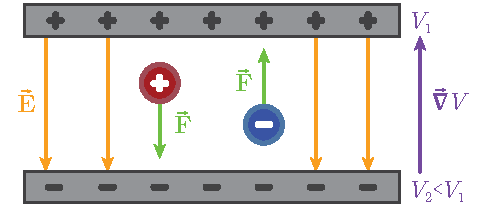
\includegraphics[width=0.6\textwidth]{images/chp3/chp3armature.pdf}
	\end{center}
	Il funzionamento di tale sistema non è dissimile, a livello puramente qualitativo, da un dipolo elettrico: tra le due piastre il campo è sostanzialmente analogo a quello sull'asse verticale congiungente i dipoli e quindi è diretto dalla piastra positiva a quella negativa.\\
	Poiché $\vba{F}=q\vba{E}$, le cariche positive saranno attratte verso la parte negativa, quelle negative verso la piastra positiva.\\
	Essendo $\grad{V}=-\vba{E}$, all'interno delle piastre il \textit{gradiente del potenziale} è un campo vettoriale diretto dalla \textit{piastra negativa a quella positiva}. Per avere tale direzione, è necessario passare da un potenziale \textit{minore} ad uno \textit{maggiore}, ossia $V_2<V_1$.
\end{examplewt}
Questo ragionamento si può anche generalizzare in altri contesti, osservando dunque che il campo elettrico è diretto dal \textbf{potenziale maggiore al potenziale minore}, e quindi
\begin{itemize}
	\item cariche \textbf{positive} si muovono verso la zona di \textbf{minor} potenziale.
	\item cariche \textbf{negative} si muovono verso la zona di \textbf{maggior} potenziale.
\end{itemize}
Ricordando inoltre che l'energia potenziale è $U=qV$, si può notare che le cariche vanno \textit{sempre}, \textit{indistintamente} dal loro segno, verso un'\textbf{energia potenziale minore}.
\paragraph{Superfici equipotenziali}
\begin{define}[Superfici equipotenziali]
	Data un sistema in cui si ha una certa funzione di potenziale $V$, le \textbf{superfici equipotenziali}\index{superfici equipotenziali} sono gli insiemi descritti dall'equazione
	\begin{equation}
		V(\vba{r})=\textrm{const}
	\end{equation}
	Le superfici equipotenziali sono sempre ortogonali, punto per punto, a $\grad{V}$ e quindi anche al campo vettoriale elettrostatico $\vba{E}$.
\end{define}
\begin{examples}~{}
	\begin{itemize}
		\item Per il potenziale della carica puntiforme,
		\begin{equation*}
			V=\frac{q}{4\pi\epsilon_0r}=\mathrm{const}\implies r=\mathrm{const}
		\end{equation*}
		le superfici equipotenziali sono circonferenze concentriche di raggio $r$, al variare di $r$:
		\begin{center}
			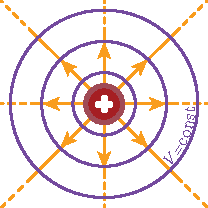
\includegraphics[width=0.35\textwidth]{images/chp3/chp3potcampocoulomb1.pdf}\hspace{20pt}
			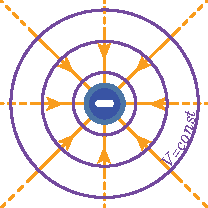
\includegraphics[width=0.35\textwidth]{images/chp3/chp3potcampocoulomb2.pdf}
		\end{center}
		\item Per il dipolo elettrico $+/-$ e quello $+/+$
		\begin{center}
			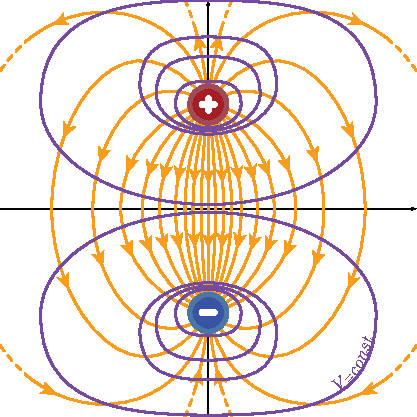
\includegraphics[width=0.45\textwidth]{images/chp3/chp3potcampodipolo1.pdf}\hspace{20pt}
			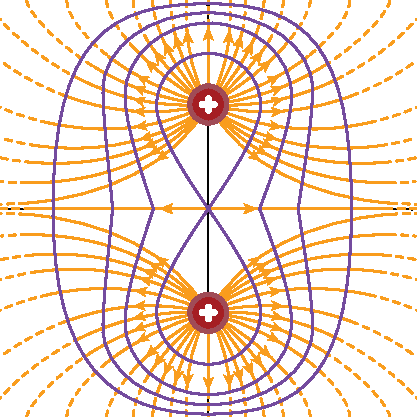
\includegraphics[width=0.45\textwidth]{images/chp3/chp3potcampodipolo2.pdf}
		\end{center}
	\end{itemize}
\end{examples}
\section{Discontinuità di campo elettrico tra superfici}
Precedentemente abbiamo ricavato il campo elettrostatico e il potenziale di volumi uniformemente carichi, come una sfera. Ci chiediamo ora quale sia il campo elettrostatico e di conseguenza il potenziale di una \textbf{superficie cava} uniformemente carica, come ad esempio una superficie sferica o un cilindro.
\paragraph{Superficie sferica uniformemente carica}
Si consideri una superficie sferica di raggio $R$ con densità superficiale costante $\sigma$. Per semplicità, poniamo il sistema di riferimento in modo che l'origine coincida con il centro della sfera.
La carica totale sulla superficie è
\begin{equation}
	q=4\pi R^2 \sigma
\end{equation}
Distinguiamo, come al solito, due casi: il campo elettrico interno ($r<R$) e quello esterno ($r>R$) alla sfera.
\begin{itemize}
	\item $\mathbf{r<R}$. Utilizziamo la \textit{legge di Gauss} su una superficie $\Sigma$ di raggio $r<R$ centrata nell'origine. Dalla definizione di flusso abbiamo che
	\begin{equation*}
		\Phi_{\Sigma}(\vba{E})=\int E(r)d\Sigma=4\pi r^2 E_r(r)
	\end{equation*}
dato che $E(r)$ è costante su $\Sigma$.
Tuttavia, poiché la carica è concentrata tutta sulla sfera di raggio $R$, la superficie $\Sigma$ \textit{non} contiene alcuna carica; pertanto, per la \textit{legge di Gauss}
\begin{equation*}
	4\pi r^2 E_r(r)=\Phi_{\Sigma}(\vba{E})=\frac{q_{int}}{\epsilon_0}=0
\end{equation*}
da cui segue che
\begin{equation}
	\vba{E}(r)=0
\end{equation}
\item $\mathbf{r>R}$. Sulla base di osservazioni precedenti, il comportamento esterno è analogo a quello di una carica puntiforme nell'origine.
\begin{equation}
	\vba{E}(r)=\frac{\sigma R^2}{\epsilon_0r^2}\vbh{u}_r=\frac{q}{4\pi\epsilon_0r^2}\vbh{u}_r
\end{equation}
\end{itemize}
Il campo elettrico, pertanto, è \textit{discontinuo} e vale
\begin{equation}
	\vba{E}(r)=\begin{cases}
		0&\text{se}\ r< R\\
		\frac{\sigma R^2}{\epsilon_0r^2}\vbh{u}_r=\frac{q}{4\pi\epsilon_0r^2}\vbh{u}_r &\text{se}\ r> R
	\end{cases}
\end{equation}
\begin{center}
	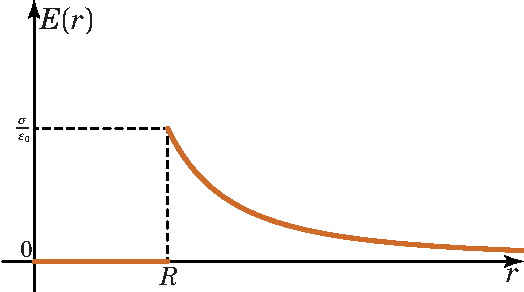
\includegraphics[width=0.75\textwidth]{images/chp3/chp3sferacavagraf1.pdf}
\end{center}
Si osserva una discontinuità pari a $\frac{\sigma}{\epsilon_0}$ tra il campo elettrico interno ed esterno alla superficie.
Data la dipendenza di $\vba{E}$ dalla sola coordinata radiale, per ottenere il potenziale è sufficiente integrare il campo elettrico rispetto ad $r$ e imporre le ben note condizioni di contorno ($V(+\infty)=0$ e continuità in $R$):
\begin{equation}
	V(r)=
	\begin{cases}
	\frac{\sigma R}{\epsilon_0}=\frac{q}{4\pi\epsilon_0 R}&\text{se}\ r< R\\
	\frac{\sigma R^2}{\epsilon_0 r}=\frac{q}{4\pi\epsilon_0 r}&\text{se}\ r> R
	\end{cases}
\end{equation}
\begin{center}
	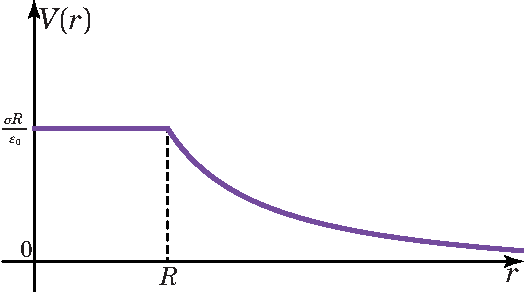
\includegraphics[width=0.75\textwidth]{images/chp3/chp3sferacavagraf2.pdf}
\end{center}
\paragraph{Superficie cilindrica uniformemente carica}\label{supcilindrounifcarica}
Si consideri una superficie cilindrica infinita e di raggio $R_0$ con densità superficiale costante $\sigma$, dove le cariche sono disposte sulla faccia laterale. Per semplicità, poniamo il sistema di riferimento in modo che l'asse $z$ passi per l'asse del cilindro.
La carica totale sulla superficie è infinita, in quanto
\begin{equation}
	q=A_{laterale} \sigma=2\pi R_0 L \sigma\underset{L\to+\infty}{\longrightarrow}+\infty
\end{equation}
Distinguiamo due casi: il campo elettrico interno ($R<R_0$) e quello esterno ($R>R_0$) al cilindro.
\begin{itemize}
	\item $\mathbf{R<R_0}$. Utilizziamo la \textit{legge di Gauss} su un cilindro $\Sigma$ di raggio $R<R_0$ con asse sull'asse $z$. Dalla definizione di flusso abbiamo che
	\begin{equation*}
		\Phi_{\Sigma}(\vba{E})=\int E(R)d\Sigma=2\pi R L E_R(R)
	\end{equation*}
	dato che $E(R)$ è costante su $\Sigma$.
	Tuttavia, poiché la carica è concentrata tutta sul cilindro di raggio $R_0$, la superficie $\Sigma$ \textit{non} contiene alcuna carica; pertanto, per la \textit{legge di Gauss}
	\begin{equation*}
		2\pi R L E_R(R)=\Phi_{\Sigma}(\vba{E})=\frac{q_{int}}{\epsilon_0}=0
	\end{equation*}
	da cui segue che
	\begin{equation}
		\vba{E}(R)=0
	\end{equation}
	\item $\mathbf{R>R_0}$. Come il campo esterno alla sfera (piena/cava) è simile al campo di Coulomb, il comportamento \textit{esterno} del cilindro cavo è analogo a quello di un filo infinito carico. Infatti, posto
	\begin{equation*}
		\lambda=\frac{q}{L}=2\pi R_0 \sigma
	\end{equation*}
	applichiamo la \textit{legge di Gauss} su un cilindro $\Sigma$ di raggio $R>R_0$ con asse sull'asse $z$:
	\begin{equation*}
		2\pi R L E_R(R)=\Phi_{\Sigma}(\vba{E})=\frac{q}{\epsilon_0}=\frac{q}{\epsilon_0}=\frac{\lambda L}{\epsilon_0}=\frac{2\pi R_0 L \sigma}{\epsilon_0}
	\end{equation*}
	segue
	\begin{equation}
		\vba{E}(R)=\frac{\lambda}{2\pi \epsilon_0 R}=\frac{\sigma R_0}{\epsilon_0 R}\vbh{u}_R
	\end{equation}
\end{itemize}
Il campo elettrico, pertanto, è discontinuo e vale
\begin{equation}
	\vba{E}(R)=\begin{cases}
		0&\text{se}\ R< R_0\\
		\frac{\sigma R_0}{\epsilon_0 R}\vbh{u}_R=\frac{\lambda}{2\pi\epsilon_0 R}\vbh{u}_R &\text{se}\ R> R_0
	\end{cases}
\end{equation}
\begin{center}
	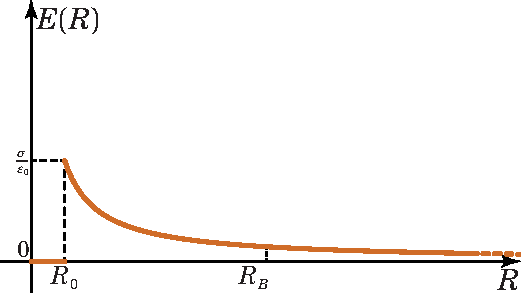
\includegraphics[width=0.7\textwidth]{images/chp3/chp3cilindrograf1.pdf}
\end{center}
Si osserva una discontinuità pari a $\frac{\sigma}{\epsilon_0}$ tra il campo elettrico interno ed esterno alla superficie.\\
Per calcolare il potenziale, notiamo che il campo dipende esclusivamente dalla coordinata radiale delle coordinate cilindriche e quindi la relazione $\vba{E}=-\grad{V}$ si trasforma in
\begin{equation*}
	E(R)=-\pdv{V}{R}
\end{equation*}
da cui
\begin{equation*}
	V(R)=-\int E(R)dR+A
\end{equation*}
con $A$ costante determinate dalle condizioni al contorno. Integrando, otteniamo
\begin{equation*}
	V(R)=
	\begin{cases}
		A&\text{se}\ R< R_0\\
		-\frac{\sigma R_0}{\epsilon_0}\log R + B=-\frac{\lambda}{2\pi\epsilon_0}\log R + B&\text{se}\ R> R_0
	\end{cases}
\end{equation*}
con $A$ e $B$ costanti.\\
Tuttavia, incappiamo in un apparente \textit{problema}: se prendiamo come punto per il potenziale nullo l'infinito, il potenziale \textit{diverge}! Non c'è da meravigliarsi di ciò, dato che questa è una situazione fisica irrealizzabile nella realtà: avendo preso un cilindro di lunghezza infinita, la distribuzione di carica si estende anche all'infinito.\\
Ricordiamo che il potenziale è determinato soltanto a meno di costanti: una scelta migliore, in questi casi, è di imporre il punto di potenziale nullo in un posto a nostra scelta. Ad esempio, prendiamo una distanza radiale \textit{arbitraria} $R_{B}$ e fissiamo $V(R_B)=0$: imponendo questa condizione novella e la solita continuità in $R=R_0$, otteniamo il potenziale continuo
\begin{equation}
	V(R)=
	\begin{cases}
		\frac{\sigma R_0}{\epsilon_0}\log \frac{R_B}{R_0}=\frac{\lambda}{2\pi\epsilon_0}\log \frac{R_B}{R_0}&\text{se}\ R< R_0\\
		\frac{\sigma R_0}{\epsilon_0}\log \frac{R_B}{R}=\frac{\lambda}{2\pi\epsilon_0}\log \frac{R_B}{R}&\text{se}\ R> R_0
	\end{cases}
\end{equation}
\begin{center}
	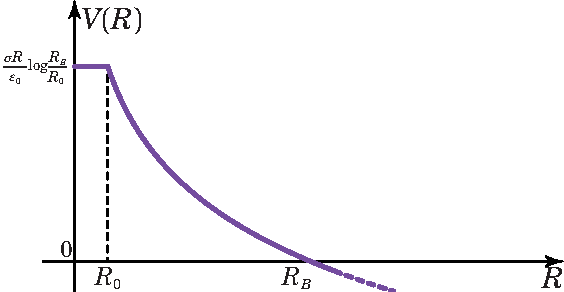
\includegraphics[width=0.7\textwidth]{images/chp3/chp3cilindrograf2.pdf}
\end{center}
Chiaramente rimarrà la divergenza del potenziale a grandi distanze, ma la \textit{scelta} effettuata garantisce almeno un punto in cui il potenziale si \textit{annulla}.
\paragraph{Il caso generale}
Sebbene l'andamento del campo elettrico nei due esempi precedenti è leggermente diverso, per entrambi i casi la discontinuità tra campo elettrico interno ed esterno in uno stesso punto è pari al valore $\frac{\sigma}{\epsilon_0}$. Non è una coincidenza fortuita, bensì possiamo mostrare che questo è \textit{sempre} così.
\begin{proposition}[Discontinuità di campo elettrico tra superfici]
	La differenza di campo elettrico tra due lati di una superficie carica è, punto per punto, pari a 
	\begin{equation*}
		\tcboxmath[colback=yellowpastellow!30!white,colframe=yelloworange!85!black,drop fuzzy shadow, nobeforeafter, math upper, tcbox raise base, enhanced]{\Delta \vba{E}(\vba{r})=\frac{\sigma}{\epsilon_0}\vbh{u}_n}
	\end{equation*}
\end{proposition}
\begin{demonstration}
	Dimostriamo tale proprietà per un foglio carico (supponiamo positivamente), dato che la superficie si può considerare almeno localmente come un foglio 
	carico.\\
	Posta una carica positiva su una faccia del foglio, ci aspettiamo che si allontani da esso ``dallo stesso lato del foglio'' a causa di un campo elettrico $\vba{E}_1$; viceversa, mettendo una particella positiva dall'altra faccia è prevedibile che la particella sarà respinta dalla superficie da quello stesso lato dalla forza generata dal campo elettrico $\vba{E}_2$, ossia dal verso opposto di $\vba{E}_1$: ci dovrà essere necessariamente una discontinuità di campo elettrico per avere questo cambio drastico di verso.
	\begin{center}
		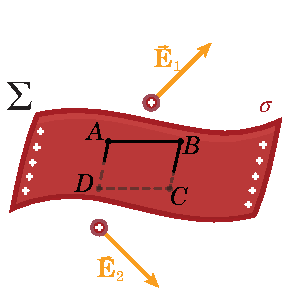
\includegraphics[width=0.35\textwidth]{images/chp3/chp3discontinuita1.pdf}
	\end{center}
	Disegniamo un circuito rettangolare $\gamma=[ABCD]$ che interseca il campo e che sia sufficientemente piccolo in modo da considerare $\vba{E}$ costante sul circuito.\\
	Dato che la circuitazione circuitazione lungo $\gamma$ è influenzata solo dalle componenti tangenziali $E_{i,t}$ e non dalle componenti perpendicolari $E_{i,n}$ al circuito, si ha
	\begin{equation*}
		0=\Gamma_{\gamma}(\vba{E})=E_{1,t}d_{AB}-E_{2,t}d_{CD}=\left(E_{2,t}-E_{1,t}\right)d_{AB}
	\end{equation*}
Da cui segue che
\begin{equation*}
	E_{2,t}=E_{1,t},
\end{equation*}
ossia che le componenti tangenziali devono essere uguali.
\begin{center}
	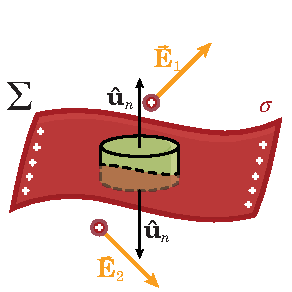
\includegraphics[width=0.45\textwidth]{images/chp3/chp3discontinuita2.pdf}
\end{center}
Consideriamo lo stesso foglio, questa volta intersecandolo con una superficie cilindrica con altezza sufficientemente piccola in modo che  il campo elettrico è considerabile costante lungo la superficie di base.\\
Calcolando il flusso e confrontandolo con quello ottenuto dalle \textit{legge di Gauss}, ricordiamo che lungo la superficie laterale esso è nullo:
\begin{equation*}
	\frac{q_{A_{base}}}{\epsilon_0}=\Phi_{\Sigma}(\vba{E})=E_{1,n}A_{base}-E_{2,n}A_{base}
\end{equation*}
Da cui segue invece
\begin{equation*}
	E_{1,n}-E_{2,n}=\frac{\sigma}{\epsilon_0}
\end{equation*}
Allora, facendo la differenza punto per punto, si ha
\begin{equation*}
	\Delta\vba{E}=\underbrace{\left(E_{1,t}-E_{2,t}\right)}_{=0}\vbh{u}_t+\underbrace{\left(E_{1,n}-E_{2,n}\right)}_{=\frac{\sigma}{\epsilon_0}}\vbh{u}_n=\frac{\sigma}{\epsilon_0}\vbh{u}_n\qedhere
\end{equation*}
\end{demonstration}
\section{Le equazioni di Maxwell per l'elettrostatica nel vuoto}
A questo punto siamo arrivati ad avere tutti gli strumenti e i risultati necessari per enunciare le \textbf{equazioni di Maxwell relative all'elettrostatica}.c Tuttavia, prima di far ciò è importante riprendere in mano alcuni risultati matematici e fisici che ci serviranno a tal scopo.
\begin{remember}~\\
		\begin{tabular}{p{0.47\textwidth}p{0.47\textwidth}}
			\begin{itemize}
				\item[1a] \textbf{Teorema della divergenza:} si consideri un volume $V\subseteq\realset^3$ compatto con bordo liscio $\partial V$. Dato un campo vettoriale differenziabile $\vba{G}$ in un intorno di $V$, allora
				\begin{equation*}
					\int_V\div{\vba{G}}=\int_{\partial V}\vba{G}\vdot \vbh{u}_nd\Sigma
				\end{equation*}
				o, equivalentemente,
				\begin{equation*}
					\int_V\div{\vba{G}}=\Phi_\Sigma\left(\vba{G}\right)
				\end{equation*}
			\end{itemize} &
			\begin{itemize}
			\item[1b] \textbf{Teorema del rotore:} si consideri una curva $\ \funz[\gamma]{\left[a,b\right]}{\realset^3}$ semplice - ossia senza intersezioni con sé stessa, chiusa e liscia a tratti; si consideri inoltre una superficie $\Sigma$ liscia tale che $\partial \Sigma=\gamma$. Dato un campo vettoriale differenziabile $\vba{G}$ in un intorno di $V$, allora
			\begin{equation*}
				\int_\Sigma\curl{\vba{G}}\vdot\vbh{u}_nd\Sigma=\oint_{\gamma}\vba{G}\vdot d\vba{s}
			\end{equation*}
			o, equivalentemente,
			\begin{equation*}
				\Phi_\Sigma\left(\curl{\vba{G}}\right)=\Gamma_\gamma\left(\vba{G}\right)
			\end{equation*}
		\end{itemize}\end{tabular}\\
		\begin{tabular}{p{0.47\textwidth}p{0.47\textwidth}}
			\begin{itemize}
				\item[2a] \textbf{Legge di Gauss:} il flusso del campo elettrostatico $\vba{E}$ attraverso un superficie \textit{chiusa} è eguale alla quantità di carica contenuta all'\textbf{interno} della superficie, comunque siano distribuite, divisa per $\epsilon_0$.
				\begin{equation*}
					\Phi_\Sigma(\vba{E})=\frac{1}{\epsilon_0}\int_{V}\rho(\vba{r})dV
				\end{equation*}
				dove $V$ è uno spazio delimitato da $\Sigma$, ossia tale che $\partial V=\Sigma$.
			\end{itemize} &
			\begin{itemize}
				\item[2b] \textbf{Circuitazione del campo elettrico nulla:} su ogni curva chiusa $\gamma$ nello spazio, la circuitazione del campo elettrostatico è nulla.
				\begin{equation*}
					\Gamma_{\gamma}(\vba{E})=0
				\end{equation*}
			\end{itemize}
		\end{tabular}
\end{remember}
\begin{theorema}[Equazioni di Maxwell per l'elettrostatica nel vuoto]
	Dato il campo elettrostatico $\vba{E}$ e una densità di carica $\rho$, valgono le seguenti relazioni:
	\begin{center}
		\begin{tabular}{p{0.22\textwidth}|c|c}
			%\multicolumn{2}{c}{\textbf{---}} \\\hline  >{\centering}
			\centering{\textbf{Nome}} &
			\textbf{Forma integrale} &
			\begin{tabular}{@{}c@{}} \textbf{Forma} \\ \textbf{differenziale}\end{tabular} \\ \hline
			
			\begin{tabular}[c]{@{}p{0.22\textwidth}@{}}	
				\\[-2mm]\textbf{Legge di Gauss per l'elettricità}\\[-2mm]~
			\end{tabular}
			&
			\begin{tabular}[c]{@{}c@{}}
				\\[-2mm]
				$\displaystyle\Phi_{\partial V}(\vba{E})=\int_{\partial V}\vba{E}\vdot\vbh{u}_nd\Sigma=\frac{q_{int}}{\epsilon_0}=\frac{1}{\epsilon_0}\int_{V}\rho dV$\\[-2mm]~
			\end{tabular} &
			\begin{tabular}[c]{@{}c@{}}
				\\[-2mm]
				$\displaystyle\div{\vba{E}}=\frac{\rho}{\epsilon_0}$\\[-2mm]~
			\end{tabular} \\ \hline
			\begin{tabular}[c]{@{}p{0.22\textwidth}@{}}	
				\\[-2mm] \textbf{Legge dell'induzione di Faraday}\\[-2mm]~
			\end{tabular} &
			\begin{tabular}[l]{@{}l@{}}
				\\[-3mm]
				$\displaystyle\Gamma_{\gamma}(\vba{E})=\oint_{\partial \Sigma} \vba{E}\vdot d\vba{s}=0$\\[-1mm]~
			\end{tabular}
			&
			\begin{tabular}[c]{@{}c@{}}
				\\[-3mm]
				$\displaystyle\curl{\vba{E}}=0$
			\end{tabular}
		\end{tabular}
	\end{center}
\end{theorema}
\begin{demonstration}
	Per ottenere la prima legge, partiamo dalla legge di Gauss
	\begin{equation*}
		\Phi_\Sigma(\vba{E})=\frac{q}{\epsilon_0}
	\end{equation*}
scritta nella sua formulazione integrale:
	\begin{equation*}
		\int_{\partial V}\vba{E}\vdot\vbh{u}_nd\Sigma=\frac{1}{\epsilon_0}\int_{V}\rho(\vba{r})dV
	\end{equation*}
Applichiamo il teorema della divergenza al primo membro:
\begin{equation*}
	\int_V\div{\vba{E}}dV=\int_V\frac{\rho}{\epsilon_0}dV
\end{equation*}
Poiché questa relazione è vera per un qualunque volume $V$ arbitrario, si deve necessariamente avere uguaglianza degli integrandi, ottenendo
\begin{equation*}
	\div{\vba{E}}=\frac{\rho}{\epsilon_0}
\end{equation*}
Per ottenere la seconda legge, partiamo dalla circuitazione nulla del campo elettrostatico
\begin{equation*}
	\Gamma_{\gamma}(\vba{E})=0
\end{equation*}
scritta nella sua formulazione integrale:
\begin{equation*}
	\oint_{\gamma}\vba{E}\vdot d\vba{s}=0
\end{equation*}
Applicando il teorema del rotore al membro non nullo:
\begin{equation*}
	\int_{\Sigma}\curl{\vba{E}}\vdot \vbh{u}_nd\Sigma=0
\end{equation*}
Poiché questa relazione è vera per una qualunque superficie $\Sigma$ arbitraria, si deve necessariamente avere che l'unico termine non dipendente dalla superficie sia sempre nullo.
\begin{equation*}
	\curl{\vba{E}}=0\qedhere
\end{equation*}
\end{demonstration}
\begin{observe}
	Mentre la prima equazione vale in generale, la seconda vale \textit{solo} in elettrostatica, considerando un campo elettrico statico e in assenza di campo magnetico.\\
	Nel caso generale, vedremo che il \textit{rotore del campo elettrico dipende dalla variazione temporale del campo magnetico}. Quando studieremo i fenomeni magnetici dipendenti dal tempo spiegheremo anche che cos'è  l'\textit{induzione} e il motivo per cui dà il nome alla legge omonima.
\end{observe}

\begin{examplewt}[Sfera uniformemente carica]
	Verifichiamo che vale la prima equazione dell'elettrostatica nel caso del campo generato da una sfera carica uniformemente:
	\begin{equation*}
		\vba{E}(r)=\begin{cases}
			\frac{\rho R}{3\epsilon_0}\vbh{u}_r&\text{se}\ r< R\\
			\frac{q}{4\pi\epsilon_0 R^2}\vbh{u}_r &\text{se}\ r> R
		\end{cases}
	\end{equation*}
	Data la divergenza di un campo in coordinate sferiche\footnote{Nella ``Raccolta Differenziata'', a pag. \pageref{DivergenzaSferiche} è possibile trovare a grandi linee il procedimento per ricavare la divergenza in coordinate sferiche.}, che ricordiamo essere
	\begin{equation*}
		\div{\vba{G}}=\frac{1}{r^2}\pdv{r}\left(r^2G_r\right)+\frac{1}{r\sin\theta}\pdv{\theta}\left(G_\theta\sin\theta\right)+\frac{1}{r\sin\theta}\pdv{G_\phi}{\phi}
	\end{equation*}
	allora si ha, per un punto \textit{esterno} alla sfera (in cui \textit{non} c'è alcuna densità di corrente) vale
	\begin{equation}
		\divergence{\vba{E}}=\div{\frac{q}{4\pi\epsilon_0 R^2}\vbh{u}_r}=\frac{1}{r^2}\pdv{r}\left(r^2\frac{q}{4\pi\epsilon_0 R^2}\right)=0
	\end{equation}
	mentre per un punto \textit{interno} alla sfera (in cui si ha una densità di corrente $\rho$) vale
	\begin{equation*}
		\div{\vba{E}}=\div{\left(\frac{\rho R}{3\epsilon_0R^2}\vbh{u}_r\right)}=\frac{1}{r^2}\pdv{r}\left(r^2\frac{\rho R}{3\epsilon_0R^2}\right)=\frac{1}{\Ccancel[red]{r^2}}\frac{\Ccancel[red]{3}\Ccancel[red]{r^2}}{\Ccancel[red]{3}\epsilon_0}=\frac{\rho}{\epsilon_0}
	\end{equation*}
\end{examplewt}
\section{L'equazione di Poisson e di Laplace}\label{EqPoissonSezione}
L'irrotazionalità del campo elettrostatico garantita dalla \textit{legge di induzione di Faraday} ci dice che, almeno localmente, è anche conservativo:
\begin{equation*}
	\curl{\vba{E}}=0\iff \exists V\colon \vba{E}=-\grad{V}
\end{equation*}
Sostituendo nella \textit{legge di Gauss}, otteniamo
\begin{equation*}
	\div{\vba{E}}=\frac{\rho}{\epsilon}\implies\div{(\grad{V})}=-\frac{\rho}{\epsilon_0}
\end{equation*}
che è un'equazione alle derivate parziali detta \textbf{equazione di Poisson}\index{equazione!di Poisson}.
\begin{equation}
	\laplacian{V}=-\frac{\rho}{\epsilon_0}
\end{equation}
Questa equazione differenziale ci descrive il potenziale in una regione dove è presente una sorgente di densità di carica $\rho$.

In una regione priva di cariche si ha $\rho\equiv0$; l'\textbf{equazione di Laplace}\index{equazione!di Laplace} descrive il potenziale in tale regione.
\begin{equation}
	\laplacian{V}=0
\end{equation}

Imponendo delle opportune \textit{condizioni di contorno}, che siano di natura \textit{fisica} o imposte come tali per \textit{convenzione}, potremmo idealmente ricavare le soluzioni di queste equazioni e determinare in modo prettamente matematico il potenziale - e di conseguenza anche il campo elettrostatico. Il problema principale è che \textit{non sempre} è possibile trovare facilmente una soluzione; tuttavia, per alcuni specifici casi, ad esempio campi che presentano delle \textit{simmetrie} interessanti, possiamo calcolare senza troppi problemi il potenziale.
\paragraph{L'equazioni di Poisson e di Laplace con simmetria sferica}\label{EquazioniPoissonSimmetriaSferica}
Consideriamo un campo a simmetria sferica, ossia dipendente esclusivamente dalla distanza radiale:
\begin{equation*}
	V(\vba{r})=V(r)\vbh{u}_r
\end{equation*}
Dato che il laplaciano in coordinate sferiche è
	\begin{equation*}
		\laplacian=\frac{1}{r^2}\pdv{r}\left(r^2\pdv{r}\right)+\frac{1}{r^2\sin\theta}\pdv{\theta}\left(\sin\theta\pdv{\theta}\right)+\frac{1}{r^2\sin^2\theta}\pdv[2]{\phi}
	\end{equation*}
allora in un punto dello spazio dove \textit{non} c'è densità di carica si ha potenziale dato dalla soluzione dell'\textit{equazione di Laplace}
\begin{equation*}
	\frac{1}{r^2}\pdv{r}\left(r^2\pdv{r}V(r)\right)=0
\end{equation*}
Facendo gli opportuni calcoli...
\begin{gather*}
	\pdv{r}\left(r^2\pdv{r}V(r)\right)=0\\
	r^2\pdv{r}V(r)=A\\
	\pdv{r}V(r)=\frac{A}{r^2}\\
\end{gather*}
... otteniamo il potenziale
\begin{equation}
	V(r)=-\frac{A}{r}+B
\end{equation}
dove $A$ e $B$ sono costanti date dalle condizioni al contorno.

In un punto dello spazio dove c'è densità di carica $\rho$ si ha potenziale dato dalla soluzione dell'\textit{equazione di Poisson}
\begin{equation*}
	\frac{1}{r^2}\pdv{r}\left(r^2\pdv{r}V(r)\right)=-\frac{\rho}{\epsilon_0}
\end{equation*}
Consideriamo il caso di $\rho$ costante, per semplicità. Facendo gli opportuni calcoli...
\begin{gather*}
	\pdv{r}\left(r^2\pdv{r}V(r)\right)=-\frac{\rho}{\epsilon_0}r^2\\
	r^2\pdv{r}V(r)=-\frac{\rho}{3\epsilon_0}r^3+C\\
	\pdv{r}V(r)=-\frac{\rho}{3\epsilon_0}r+\frac{C}{r^2}\
\end{gather*}
... otteniamo il potenziale
\begin{equation}
	V(r)=-\frac{\rho}{6\epsilon_0}r^2-\frac{C}{r}+D
\end{equation}
dove $A$ e $B$ sono costanti date dalle condizioni al contorno.
\begin{examplewt}[Sfera uniformemente carica]
	Il campo elettrostatico della sferica uniformemente carica di raggio $R$ è un campo a simmetria radiale, pertanto il potenziale soddisfa, all'interno e all'esterno della sfera, le equazioni di Poisson e Laplace trovate prima.
	\begin{equation}
		V(r)=
		\begin{cases}
			-\frac{\rho}{6\epsilon_0}r^2-\frac{C}{r}+D&\text{se}\ r< R\\
			-\frac{A}{r}+B&\text{se}\ r> R
		\end{cases}
	\end{equation}
	Ci basta ora imporre le condizioni al contorno.
	\begin{itemize}
		\item Per \textit{convenzione}, si suppone che il potenziale per $r\to\infty$ tenda a $0$, dato che il campo elettrico si considera trascurabili a enormi distanze.\footnote{Questo è lecito farlo perché lo \textbf{zero del potenziale} è arbitrario, grazie al fatto che il potenziale stesso è definito a meno di costanti: sostanzialmente, come decido di misurare il potenziale è una scelta di chi studia il sistema, anche se generalmente ci sono motivi fisici (come in questo caso) o geometrici per fare una certa scelta. Ciò non significa, tuttavia, che tale scelta è \textit{insignificante}, dato che \textit{ogni} valore del potenziale deve essere misurato tenendo conto di tale zero.}
		\begin{equation*}
			\lim_{r\to+\infty}V(r)=0
		\end{equation*}
		Imponendo ciò, si trova
		\begin{equation*}
			B=0
		\end{equation*}
		\item Quando siamo a grandi distanze, la sfera carica uniformemente è assimilabile ad una carica puntiforme, pertanto l'altra condizione al limite è che il campo elettrico della sfera all'esterno sia quello della sfera; da ciò è necessario imporre 
		\begin{equation*}
			A=-\frac{q}{4\pi\epsilon_0}
		\end{equation*}
	\end{itemize}
	\begin{itemize}
		\item Sulla base della continuità del potenziale, sul dominio del campo elettrico il potenziale si considera \textit{finito}, pertanto poniamo
		\begin{equation*}
			C=0
		\end{equation*}
		in modo da togliere il termine $\frac{1}{r}$, che renderebbe il potenziale infinito in $r=0$.
		\item Per garantire la continuità del potenziale si deve imporre
		\begin{equation*}
			V_{interno}(R)=V_{esterno}(R)
		\end{equation*}
			Risolvendo l'equazione
		\begin{equation*}
			-\frac{\rho}{6\epsilon_0}R^2+D=\frac{q}{4\pi\epsilon_0R}\implies D=\frac{q}{4\pi\epsilon_0R}+\frac{\rho}{6\epsilon_0}R^2
		\end{equation*}
	\end{itemize}
Il potenziale complessivo è unico ed è
\begin{equation}
	V(r)=
	\begin{cases}
		\frac{\rho}{6\epsilon_0}\left[R^2-r^2\right]+\frac{q}{4\pi\epsilon_0R}=\frac{\rho}{6\epsilon_0}\left[R^2-r^2\right]+\frac{\rho R^2}{3\epsilon_0}&\text{se}\ r< R\\
		\frac{q}{4\pi\epsilon_0r}=\frac{\rho R^3}{3\epsilon_0r}&\text{se}\ r> R
	\end{cases}
\end{equation}
\end{examplewt}
\paragraph{L'equazione di Laplace con simmetria cilindrica}
Consideriamo un campo a simmetria cilindrica, ossia dipendente esclusivamente dalla distanza assiale:
\begin{equation*}
	V(\vba{r})=V(R)\vbh{u}_R
\end{equation*}
Dato che il laplaciano in coordinate cilindriche è
\begin{equation*}
	\laplacian=\frac{1}{R}\pdv{R}\left(R\pdv{R}\right)+\frac{1}{R^2}\pdv[2]{\theta}+\pdv[2]{z}
\end{equation*}
allora in un punto dello spazio dove non c'è densità di carica si ha potenziale dato dalla soluzione dell'\textit{equazione di Laplace}
\begin{equation*}
	\frac{1}{r}\pdv{r}\left(r\pdv{r}V(r)\right)=0
\end{equation*}
Facendo gli opportuni calcoli...
\begin{gather*}
	\pdv{r}\left(r\pdv{r}V(r)\right)=0\\
	r\pdv{r}V(r)=A\\
	\pdv{r}V(r)=\frac{A}{r}\\
\end{gather*}
... otteniamo il potenziale
\begin{equation}
	V(r)=A\log{r}+B
\end{equation}
dove $A$ e $B$ sono costanti date dalle condizioni al contorno.
%TODO: add soluzione poisson?

